\documentclass[letterpaper, 10pt, twocolumn, reqno]{amsart}
%\documentclass[letterpaper, 10pt, reqno]{amsart}

\usepackage[margin=1in]{geometry}
\usepackage{mathpazo, flushend}
% packages
\usepackage{amsmath, amsfonts, amssymb, bm, enumerate, url} %, flushend}
\usepackage[boxruled, vlined, linesnumbered]{algorithm2e}
\usepackage[usenames, dvipsnames]{color}
\usepackage[pdftex, xetex]{graphicx}
\usepackage[font={small}]{caption}
\usepackage{float, colortbl, tabularx, multirow, subcaption, environ, wrapfig}
\usepackage{pgf, tikz}
\usetikzlibrary{arrows,automata}
\usepackage[normalem]{ulem}

\usepackage[bookmarks=true]{hyperref}
%\usepackage[hyperpageref]{backref}
\hypersetup{
colorlinks=true, linkcolor=red, citecolor=blue, filecolor=magenta, urlcolor=blue
%linkcolor=black, citecolor=black, filecolor=black, urlcolor=black
}

\usepackage{url, natbib}

% macros
\definecolor{darkgreen}{rgb}{0,0.6,0} \newcommand{\dg}{\color{darkgreen}}
\definecolor{fullred}{rgb}{0.85,.0,.1} \newcommand{\fr}{\color{fullred}}
\definecolor{brown}{rgb}{0.65,0.16,0.16} \newcommand{\br}{\color{brown}}
\definecolor{orange}{rgb}{1,0.5,0} \newcommand{\oran}{\color{orange}}
\newcommand{\bl}{\color{blue}}
\newcommand{\pcmargin}[2]{{\dg #1}\marginpar{\tiny\noindent{\raggedright{\oran[PC]}\bl{ #2} \par}}}
\newcommand{\pc}[2]{\pcmargin{#1}{#2}}


%\newcommand{\myclearpage}{\clearpage}
\newcommand{\myclearpage}{}

% math macros
\newcommand{\abs}[1]{\ensuremath \left| #1 \right|}
\newcommand{\norm}[1]{\ensuremath \lVert#1\rVert}
\newcommand{\given}{\, \vert \,}
\renewcommand{\cal}[1]{\ensuremath \mathcal{#1}}
\newcommand{\qed}{\hfill \mbox{\raggedright \rule{0.1in}{0.1in} } }

\newcommand{\aeq}[1]{\begin{align} #1 \end{align}}
\newcommand{\aeqs}[1]{\begin{align*} #1 \end{align*}}
\newcommand{\beq}[1]{\begin{equation}#1\end{equation}}
\newcommand{\beqs}[1]{\begin{equation*}#1\end{equation*}}
\newcommand{\trm}[1]{\ensuremath \textrm{#1}}
\newcommand{\enum}[2]{\begin{enumerate}[#1]{#2}\end{enumerate}}
\newcommand{\ilist}[1]{\begin{itemize}{#1}\end{itemize}}
\newcommand{\ag}[1]{\ensuremath \left\langle#1\right\rangle}
\newcommand{\bee}{\begin{enumerate}}
\newcommand{\eee}{\end{enumerate}}
\newcommand{\bmat}[1]{\begin{bmatrix}#1\end{bmatrix}}
\newcommand{\mpage}[2]{\begin{minipage}{#1}#2\end{minipage}}
\newcommand{\la}{\leftarrow}
\newcommand{\ra}{\rightarrow}

\usepackage{theorem}
\newtheorem{theorem}{Theorem}
\newtheorem{proposition}[theorem]{Proposition}
\newtheorem{lemma}[theorem]{Lemma}
\newtheorem{corollary}[theorem]{Corollary}
\newtheorem{problem}[theorem]{Problem}
%\theoremstyle{definition}
\newtheorem{definition}[theorem]{Definition}
\newtheorem{example}[theorem]{Example}
\newtheorem{note}[theorem]{Note}
\newtheorem{remark}[theorem]{Remark}
%\theoremstyle{plain}
\newtheorem{assumption}[theorem]{Assumption}


%\usepackage[marginal]{showlabels}
%\renewcommand{\showlabelfont}{\footnotesize\slshape\color{brown}}

\linespread{1.02}

\newcommand{\algsize}{\footnotesize}
\setlength{\floatsep}{0.0in}
\setlength{\textfloatsep}{0.0in}
\setlength{\intextsep}{0.0in}
\setlength{\belowcaptionskip}{0.05in}
\setlength{\abovecaptionskip}{0.05in}
\setlength{\abovedisplayskip}{0.05in}
\setlength{\belowdisplayskip}{0.05in}

\graphicspath{{../fig/}}

\title{Column Generation Techniques in Air Transportation}
\author{Pratik Chaudhari$^*$}
\thanks{$^*$ Laboratory of Information and Decision Systems, MIT.\newline
Email: \href{pratik.ac@gmail.com}{pratik.ac@gmail.com}}
\date{May 10, 2014}

\begin{document}
\maketitle

{
\small
\textbf{\emph{Abstract:}}
This project discusses column generation techniques for problems in airline scheduling. It presents a branch and price based algorithm that uses column generation for solving the integrated crew pairing and maintenance routing problems. Along the way, we also discuss column generation for canonical problems such as the cutting stock problem and resource constrainted shortest path. We also present results of an implementation on randomized instances of these problems.
}
%\vspace*{-0.1in}

\section{Introduction}
\label{sec:intro}


Modern day problems in operations research such as multi-commodity flow problems~\cite{barnhart2000using}, crew pairing~\cite{anbil1998column} and fleet assignment in
airline operations~\cite{barnhart1998flight}, even optimization problems from other fields such as graph partiting for VLSI circuits \cite{vanderbeck1994thesis}, maximum satisfiability problems~\cite{hansen1998mixed}, graph coloring~\cite{mehrotra1996column} etc. are enormously large.
Most of them are in fact mixed integer programs (MIPs) with millions of variables and contraints that often require good linear programming (LP)
relaxations. In such situations, we cannot even solve the LP relaxations in reasonable time.

A defining characteristic of most of the examples is however that only few variables take part in the optimal solution. In such cases, approaches that
incrementally add new variables (columns) to the solution without considering them all at once stand a chance to perform efficiently. A number of different
ideas such as branch and cut, branch and price etc. exist to tackle these issues. We will focus here on a technique known as column generation~\cite{desrosiers2005primer}.

Consider the crew pairing or fleet assignment problems in airline scheduling. They are typically formulated as constraints on sequences of flights using a resource, e.g, crew or aircrafts. Although the number of constraints is huge, the problem can be made tracktable if we automagically good, feasible sequences of flights. Column generation involves optimizing the original problem using constraints on these feasible paths. Let us note that the fundamental idea of generating columns as needed while solving a linear program is quite old, it was first proposed by~\cite{dantzig1960decomposition} almost five decades ago. The cutting stock problem, which we will explore in detail in this paper was in fact one of the first problems where column generation was demonstrated~\cite{gilmore1961linear,gilmore1963linear}.

More formally, if the entire set of variables (columns) is unnecessary for the solution, the basis variables (cf.\@ simplex algorithm) can be generated as
needed. This is akin to solving a \emph{restricted master problem} in conjunction with smaller sub-problems, also known as \emph{pricing problems}.
This sub-problem, roughly speaking, finds the new basis variable by minimizing the reduced cost of each new variable using the dual variables in the restricted problem. We iterate to construct a new master problem by adding
this new variable to the optimization. The efficacy of column generation (also known as \emph{branch-and-price}~\cite{barnhart1998branch} for integer programs) hinges on an efficient solution to the pricing problem. For example, in
fleet assignment, maintenance routing and crew scheduling, the master problem is a \emph{set-cover problem} while the pricing problem is form of \emph{shortest path problem} which can be easily solved using dynamic programming.
Various similar problems like constrained or multi-label shortest path problems are viable candidates for sub-problems in branch-and-price methods.
After giving a brief overview of the algorithm, we will demonstrate an implementation of column generation techniques on canonical problems such as \emph{resource-constrained shortest path} and \emph{cutting-stock problem}. The key idea here is to express, e.g., the shortest path problem, not as a combination of individual arcs, but instead as a decision variable for whether a particular sub-path is included in the shortest path or not.

Now consider the problem of aircraft scheduling, which we define to be the combination of four sub-problems, viz., schedule design, fleet assignment, maintenance routing and crew pairing. The sheer size of each of these individual problems makes it almost impossible to solve the combined problem of aircraft scheduling, even for a small airline. Practically however, there are huge advantages to be gained in terms of optimality or even robustness if we can solve the combined problem. Due to the large number of constraints, it is a promising domain for techniques like branch-and-price. In particular, we will focus on integrating aircraft maintenance and crew pairing. As suggested in~\cite{cohn2003improving}, elements of the two problems can be integrated to ensure that only the maintenance routings that relevant to the crew scheduling problem are considered. The key idea in this approach is the notion of \emph{short connect}, which are routings that can be realized only if the crew stays on the aircraft. Evidently, a set of short connects can represent numerous different routings, which is crucial for a quick solution to the problem. We will present the integrated formulation, formulate column generation procedures for the problem and motivate a branch and price based algorithm for solving both maintenance routing and crew pairing together.

The organization of this paper is as follows --- In Sec.~\ref{sec:column_generation}, we introduce two canonical problems, the cutting stock problem and the resource constrained shortest path problem and formulate column generation procedures for these. Sec.~\ref{sec:branch_and_price} discusses the branch and price framework and introduces the crew pairing and maintenance routing problems along with their solution procedures. Sec.~\ref{sec:integrated_model} describes the integrated problem of crew pairing and maintenance routing. We discuss a branch and price based algorithm for solving the integrated problem. Sec.~\ref{sec:examples} shows results of example implementations of column generation on a few simple problems while we conclude in Sec.~\ref{sec:summary}.

\section{Column Generation}
\label{sec:column_generation}

This section introduces column generation for solving large linear programs using the cutting-stock problem and resource-constrainted shortest path as examples. We also describe the simplex algorithm and the dual problem formulation, this will be help us to motivate as well as introduce notation for column generation.

\subsection{Linear programs: Standard form}
\label{ssec:lp_standard}

The material here is presented from~\cite{bertsimas1997introduction}. We will assume that the linear program is given to us in the standard form as follows:
\aeq{
    \trm{minimize}\ &c' x, \notag \\
    \trm{subject to}\ & Ax = b, \notag \\
    & x \geq 0.
    \label{eqn:lp_standard_form}
}
where $c \in \reals^n$ is the cost-vector, $A = [a_{ij}] \in \reals^{m \times n}$ is the constraint matrix with $m$ constraints and $b \in \reals^m$. The columns of $A$, which we denote by $A_1, \ldots, A_n$ are also known as the resource vectors while $b$ is the target vector; motivated from
$$\sum_{i=1}^n A_i x_i =b.$$
%So in the standard form, we wish to synthesize $b$ using a non-negative amount, $x_i$, of each resource $A_i$.
Note that a different form of linear program, e.g., with inequality constraints can be easily converted to the standard form.
% as follows,
% \clist{
%     \item if $x_i$ is unrestricted, write it as $x_i = x_i^+ - x_i^-$ where both $x_i^+, x_i^- \geq 0$;
%     \item construct slack variables for inequality constraints, i.e., if $\sum_{j=1}^n a_{ij} x_j \leq b_i$, we use
%     $$\sum_{j=1}^n a_{ij} x_j + s_i = b_i, \quad s_i \geq 0;$$
%     \item finally, note that a maximization is just another minimization problem with a negative cost vector $c$.
% }
Let $P = \cbrac{x \given Ax \geq b, -Ax \geq -b, x \geq 0}$ be a polyhedron, note that $P$ is the space of feasible candidates for Prob.~\eqref{eqn:lp_standard_form}.

\subsection{Simplex algorithm}
\label{ssec:simplex}
The simplex algorithm is based upon the observation that the optimal solution always lies on the corners of $P$. Note that since $b \in \reals^m$, if the feasible solution $x$ were of length $m$, we can just invert the corresponding rows and obtain $x$. To that end, if $x$ is a \emph{basic feasible solution}, let $B_I = \cbrac{B_1, \ldots, B_m}$ be the indices of the basic variables, i.e, $x_j = 0$ for all other indices. Let $B = \bmat{A_{B_1}, \ldots, A_{B_m}}$ be the corresponding basis matrix. we thus have,
$$
x_B = B^{-1} b
$$
where $x_B = \bmat{x_{B_1}, \ldots, x_{B_m}}$.
Let us consider moving away from $x$ to a new vector $x + \th d$ by selecting some new variable $x_j$ and making it non-zero, i.e, $d_j = 1$ for some $j \notin B_I$. Since $A(x+\th d) = b$, we need $A d = 0$ which implies
$$
0 = A d = \sum_{i=1}^n A_i d_i = \sum_{i=1}^m A_{B_i} d_{B_i} + A_j = B d_B + A_j.
$$
Since $B$ is invertible, we get $d_B = -B^{-1} A_j$. Note that for a small $\th$, the feasiblity is still maintained as we move away from $x_B$ towards $x_B + \th d$. Also, the rate of cost change by this move is
\beq{
\bar{c}_j = c_j + c_B' d_B = c_j - c_B' B^{-1} A_j
\label{eqn:reduced_cost}
}
which is known as the ``reduced cost'' of variable $x_j$. In other words, $\bar{c}_j$ is the change in cost incurred after a unit increase in the variable $x_j$. Of course, if this is positive for all variables in the problem, we know that we have found the solution.

% The simplex algorithm then starts with a basic feasible solution and iteravtively adds new variables to this set. While doing so, we would like to pick a $\th$ s.t. $x+\th d$ is a large step, i.e.,
% $$
% \th^* = \max \cbrac{\th \given x + \th d \in P}.
% $$
% It can be shown that $\th^*$ has a simple formula
% $$
% \th^* = \min_{i \in [m],\ d_{B_i} < 0}\ \rbrac{- \f{x_{B_i}}{d_{B_i}}}.
% $$
% Thus the iteration of the simplex algorithm are simple.
% \enum{
%     \item Start with $A_B$ and  current basic solution $x$, compute the reduced costs $\bar{c}_j = c_j - c_B' B^{-1} A_j$ for all non-basic variables $x_j$; if all
%     $\bar{c}_j \geq 0$, $x$ is optimal solution, else pick some $j$ with $\bar{c}_j < 0$.
%     \item Calculate $\th^* = \min_{i \in [m],\ d_{B_i} < 0}\ \rbrac{- \f{x_{B_i}}{d_{B_i}} }$. If there is no $i$ s.t. $d_{B_i} < 0$, the optimal cost is $-\infty$.
%     \item Let $l$ be the minimizing index in step 2., form a new basis by replacing $A_{B_l}$ with $A_j$ and set ${x_j \la \th^*}$ and $x_{B_i} \la x_{B_i} - \th^* d_{B_i}$.
%  }
% The above algorithm can be made much more efficient by passing information about dual variables in consecutive steps.

% \subsection{Dual problem}
% \label{ssec:dual}

% We can write the Prob.~\eqref{eqn:lp_standard_form} as
% \aeqs{
%     \trm{minimize}\ & c'x + p'(b - Ax), \\
%     \trm{subject to}\ & x \geq 0.
% }
% where $p \in \reals^m$ is the Lagrange multiplier. This new problem has fewer constraints and hence by definition,
% \aeqs{
% g(p) = \min_{x \geq 0} \sqbrac{c'x + p'(b-Ax)} &\leq c'x^* + p'(b-Ax^*) \\
% &=c' x^*.
% }
% Here $x^*$ is the optimal solution of Prob.~\eqref{eqn:lp_standard_form} (also known as the ``primal'') and the last equality is true because $p$ at optimality is such that all constraints are satisfied. The new problem,
% \aeqs{
%     \trm{maximize}\ &g(p), \\
%     \trm{subject to}\ &\trm{no constraints}
% }
% thus searches for the best lower bound of the primal. Note that
% \aeqs{
% g(p) = \begin{cases}
% p' b \quad & \trm{if}\ c' \geq p'A\\
% -\infty, \quad & \trm{otherwise}.
% \end{cases}
% }
% Thus, the ``dual'' problem of Prob.~\eqref{eqn:lp_standard_form} is
% \aeq{
%     \trm{maximize}\ \quad& p' b, \notag\\
%     \trm{subject to}\ \quad& p'A \leq c'.
% }
% Dual problems are important for many reasons, viz., (i) the dual of a dual is the primal, (ii) dual solution is a lower bound for the primal's cost and finally, (iii) if the primal has a solution, so does the dual, and moreover, their costs are the same.

\subsection{Cutting-stock problem}
\label{ssec:col_gen_cutting_stock}

Consider a paper mill with a number of rolls of paper of fixed width available to it. Different customers want different numbers of rolls of various-sized widths. The problem is to them efficiently cut ``patterns'' in each roll of paper so as to avoid waste. To get an idea of the magnitude of the problem, note that European paper mills produced a total turnover of almost $\$ 75$ million in 2012 and hence saving even 1\% of this is a significant advantage.

Let the width of each roll be $W$ and $m$ customers want $n_i$ rolls each of width $w_i$. If $K$ is the number of rolls available, let $y_k = 1$ if a roll $k \in [K]$ is cut and zero otherwise. Let $x_i^k$ be the number of times item $i$ is cut on roll $k$. We then have the following formulation.
\aeq{
    (P_1) \quad \min &\sum_{k \in [K]} y_k, \notag \\
    \trm{s.t.}\ & \sum_{k \in [K]} x_i^k \geq n_i \quad \forall\ i \in [m], \qquad \trm{(demand)}\notag\\
    & \sum_{i=1}^n w_i x_i^k \leq W y_k \quad \forall k \in [K],\quad \trm{(width of roll)} \notag\\
    &x_i^k \in \integers_+, y_k \in \cbrac{0,1}.
    \label{eqn:cutting_stock_ip}
}
Note that the above problem has $Kn + K$ variables and $(n+K)$ constraints and since it is an integer program, solving it for even small values of $K, n$ is expensive. The real reason for this is that the LP relaxation of this problem is bad. Note that
\beq{
\sum_k y_k \geq \f{1}{W} \sum_k \sum_i w_i\ x_i^k \geq \f{1}{W} \sum_i n_i\ w_i
\label{eqn:csp_lp_relax_bound}
}
which is a naive bound and says that the number of rolls needed is simply the sum of all demands divided by $W$. Let use pose the problem in a different way as follows.

We call the set of distinct cuts of a roll as a pattern, i.e., if $W=100$, and we make 4 cuts of $w_1 = 25$ each, we generate a patterm $\{ w_1, w_1, w_1, w_1 \}$. If on the other hand, we make one cut of $w_1 =25$ and two of $w_2 = 35$, we generate a pattern $\{ w_1, w_2, w_2 \}$. Let $x_j$ be the number of times a pattern $j$ is used. Let $a_{ij}$ be the number of times item $i$ is cut in pattern $j$. Consider then, the new problem --
\aeq{
    (P_2) \quad \min &\sum_{j=1}^n x_j, \notag \\
    \trm{s.t.}\ & \sum_{j=1}^n a_{ij} x_j \geq n_i \quad \forall\ i \in [m], \qquad \trm{(demand)} \notag\\
    &x_j \in \integers_+, j \in [n].
    \label{eqn:cutting_stock_pattern_ip}
}
where $n$ is the number of valid patterns, i.e., ones that satisfy $\sum_{i=1}^m w_i a_{ij} \leq W$. Note that the new problem is also an IP and moreover, it contains a huge number of variables, almost $m \choose k$, where $k$ is the average number of items in a pattern. However, let's look at its LP relaxation. We replace the integrality constraints with
$$
x_j \in \reals_+,\quad j \in [n].
$$
We call the new problem, the ``Linear Programming Master (LPM)''; the solution to this could very well be non-integral, since we have $\geq$ in the constraints we can generate a feasible, integral solution by rounding up. It has a large number of variables but only $m$ constraints. Use now use the simplex algorithm from Sec.~\ref{ssec:simplex} to solve this LP.

The main idea of column-generation is that most of variables are zero, i.e., they do not form the basis (since the basis has only as many variables as constraints). Hence, we only need a small subset of all the variables to form the solution. How do we leverage this observation? Let us start with a subset $\cP \subset [n]$ of columns of LPM and call it the ``Restricted Linear Programming Master (RLPM)''and now look at its dual problem.
\aeq{
    \trm{maximize}\ &\sum_{i=1}^m n_i \pi_i, \notag \\
    \trm{subject to}\ & \sum_{i=1}^m \a_{ij} \pi_i \leq 1, \quad j \in \cP, \notag\\
    &\pi \geq 0, \quad i \in [m].
    \label{eqn:cutting_stock_dual_rlpm}
}
Let $\hat{\pi}$ be the optimal solution to the dual problem. The reduced cost of column $j$ in that case is given by simply
$$
1  - \sum_{i=1}^m a_{ij}\ \hat{\pi}_i.
$$
The variable with the best reduced cost, i.e., which we absolutely must include in the primal is to find
$$
\min \cbrac{1  - \sum_{i=1}^m a_{ij}\ \hat{\pi}_i \given j \in [n] \setminus \cP}
$$
which is still expensive to do since we need to enumerate all the possible patterns. However, it is another optimization problem, and a very famous at that. This problem, which we will call as the ``sub-problem'' (or the ``pricing problem'') is a Knapsack problem, i.e.,
\aeq{
    \max \quad &\sum_{i=1}^m \hat{\pi}_i y_i, \notag \\
    \trm{s.t.}\ \quad & \sum_{i=1}^m w_i\ y_i \leq W, \notag\\
    & y_i \in \integers_+, i \in [m].
    \label{eqn:cutting_stock_sub_problem}
}
Knapsack is one of the ``easy'' NP-hard problems and can be solved in $\bigo(mW)$ time by dynamic programming. We thus have a strategy for solving the cutting-stock problem as follows.
\enum{
    \item Start with some initial columns of LPM, e.g., use a simple pattern to cut rolls into $\ceil{W/w_i}$ pieces of $w_i$. $A = [a_{ij}]$ in Prob.~\eqref{eqn:cutting_stock_pattern_ip} is thus diagonal.
    \item repeat until all reduced costs are non-negative
        \enum{
            \item Solve RLPM and let $\hat{\pi}$ be the dual variables
            \item Find a new column as the solution of knapsack pricing problem with the most negative reduced cost
            \item Add new column to RLPM
        }
}

Note that this procedure only yields a solution to LPM, i.e., the relaxed problem of Prob.~\eqref{eqn:cutting_stock_pattern_ip}. In order to get an integer solution, observe that
$$
\sum_{j=1}^n a_{ij} \ceil{x_j} \geq \sum_{j=1}^n a_{ij} x_j \geq n_i
$$
which means that the rounded-up solution is also a feasible solution for Prob.~\eqref{eqn:cutting_stock_pattern_ip}. But of course, this rounded-up solution is not optimal, to obtain the optimal solution to the original IP, we have to take recourse to ``branch and bound'', which is a technique for solving general integer linear programs. In the next section, we discuss this procedure and motivate the ``branch and price'' framework which uses column generation in addition to branch and bound.

\subsection{Resource constrained shortest path (RCSP)}
\label{ssec:rcsp}

\begin{figure}
\centering
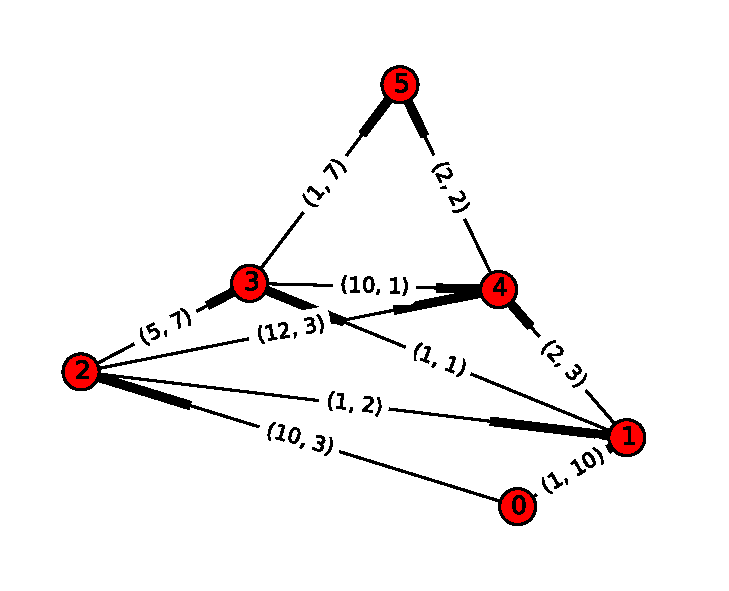
\includegraphics[width=0.8 \columnwidth]{roadnet}
\caption{Time constrained shortest path problem. The tuples on edges denote $(c_{ij}, t_{ij})$ where $c_{ij}$ is the cost for edge $(i,j)$ and $t_{ij}$ is the time duration of crossing that edge.}
\label{fig:rcsp}
\end{figure}

Let us briefly discuss another classic application of column generation. Consider the network shown in Fig.~\ref{fig:rcsp}, let $c_{ij}$ be the cost of going from node $i$ to node $j$ in $t_{ij}$ time units. In the RCSP problem, we would like to find the shortest path from say 1 to 6, with total duration of, say less than 14. It can be written as the following optimization problem.
\aeq{
    \min\ \sum_{(i,j) \in E}\ &c_{ij}\ x_{ij},\\
    \trm{s.t.}\ \sum_{(1,j) \in E} x_{1j} &= 1, \\
    \sum_{j:(i,j) \in E} x_{ij} &= \sum_{j:(j,i) \in E}\ x_{ji} \quad \forall i, \\
    \sum_{i:(i,6) \in E}\ x_{i6} &= 1,\\
    \sum_{(i,j) \in E}\ t_{ij}\ x_{ij} &\leq 14, \label{eqn:rcsp_resource}\\
    x_{ij} &\in \cbrac{0,1} \quad \forall\ (i,j) \in E.
    \label{eqn:rcsp}
}
This problem looks very much like a shortest path problem (which are easy to solve using dynamic programming), except the constraint~\eqref{eqn:rcsp_resource}. In fact, no polynomial time solution to the above problem is likely, it is NP-hard. We can however employ column generation here by leveraging a key result in network flow theory.

Define variables $x_{pij}$ to be 1 if $(i,j) \in E$ exists on a path $p \in P$ of the network. We can express the original variables as
\aeqs{
x_{ij} &= \sum_{p \in P}\ x_{pij}\ \l_p \quad (i,j) \in E,\\
\sum_{p \in P}\ \l_p &= 1,\\
\l_p &\geq 0 \quad \forall p \in P.
}
The Restricted Master Problem can now be written as follows
\aeq{
    \min\ \sum_{p \in P}\ &\sqbrac{\sum_{(i,j) \in E}\ c_{ij}\ x_{pij}}\ \l_p\\
    \trm{s.t.}\ \sum_{p \in P}\ &\sqbrac{\sum_{(i,j) \in E}\ t_{ij}\ x_{pij}}\ \l_p \leq 14, \label{eqn:rcsp_rlpm_resource}\\
    \sum_{p \in P}\ \l_p &= 1,\\
    \sum_{p \in P}\ x_{pij}\ \l_p &= x_{ij} \quad (i,j) \in E, \label{eqn:rcsp_rlpm_flow}\\
    \l_p &\geq 0 \quad \forall p \in P,\\
    x_{ij} &\in \cbrac{0,1} \quad \forall\ (i,j) \in E.
    \label{eqn:rcsp_rlpm}
}
where $P$ is a subset of the set of all paths that start at 1 and end at 6.
Roughly, $\l_p$ is the cost of path $p$ and its coefficient in \eqref{eqn:rcsp_rlpm_resource} is its time duration. As always, we start with the LP
relaxation of the above RLPM. If we remove the intergality constraints on $x_{ij}$, we can also get rid off constraints in \eqref{eqn:rcsp_rlpm_flow}. Let $\hat{\pi}$ be the duals of this problem. To find a new path $p' \notin P$, we formulate the pricing problem that minimizes the reduced cost as follows
\aeq{
    \min \sum_{(i,j) \in E}\ c_{ij}\ x_{pij} - \hat{\pi}_1 \rbrac{\sum_{(i,j)\in E} t_{ij}\ x_{pij}} - \hat{\pi}_0 \\
    \min \sum_{(i,j)\in E} \rbrac{c_{ij} - \hat{\pi}_1\ t_{ij}}\ x_{ij} - \pi_0
    \label{eqn:rcsp_sub_problem}
}
for a path that again joins 1-6 in the network. This is simply the usual shortest path problem that can be solved in $\bigo(n \log n)$ time! This is however an example where we can ``round up'' the solution, we have to embed a branch and bound strategy in the algorithm in addition to column generation. In Sec.~\ref{sec:examples} we provide results of computational experiments on both the cutting stock problem and the resource constrained shortest path problem.

\section{Branch and Price}
\label{sec:branch_and_price}

\subsection{Branch and bound}
\label{ssec:branch_and_bound}

Let us construct a simple procedure to solve general MIPs. We first construct
the relaxation and solve it iteratively by branching off non-integral solutions to successive relaxations. The idea is that the solution of a
relaxed LP, by definition, is a lower bound on the optimal cost of the MIP. Say $\hat{x}$ be the current cost. If the solution is integral, we are done. If not, we pick any non-integral variable in the solution, say $\hat{x}_i = 4.2$ and create two branches $\hat{x}_i \leq 4$ and $\hat{x}_i \geq 5$. The tree
is explored in a breadth-first manner until we get a fully integral solution. We can also prune certain branches by noting that if the solution of the
relaxed LP at some node is less than the current minimum solution, we do not need to explore that branch downwards. We use a priority queue to sort the nodes of the branch-and-bound algorithm by their LP relaxation lower bounds and pop from this queue at every iteration. Typically, one might also construct an upper bound to guide the search.
%
The final search procedure is as shown in Alg.~\ref{alg:bnb}.
\IncMargin{0.04in}
\begin{algorithm}[!h]
\footnotesize
$J_l$: LP relaxation of original problem\;
$J_u$: upper bound with integer solution (possibly heuristic)\;
$J^* \la J_u$: incumbent best solution\;
\vspace{0.05in}
\While{nodes in tree}
{
    \enum{
    \item solve current LP, compute duals
    \item update lower bound $J_l$
    \item If solution $J_c$ is fractional,
        \begin{enumerate}[(a)]
        \item if $J_c \geq J_u$, discard node
        \item if $J_c < J_l$, create two new nodes (branch)
        \end{enumerate}
    \item If integral solution,
        \begin{enumerate}[(a)]
        \item if $J_c < J_u$, update upper bound
        \item discard node
        \end{enumerate}
    }
}
\caption{Branch and bound}
\label{alg:bnb}
\end{algorithm}
\DecMargin{0.04in}

% \begin{figure}
% \centering
% 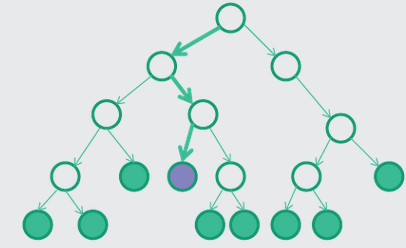
\includegraphics[width=0.8 \columnwidth]{bnb}
% \caption{Branch and bound search tree}
% \label{fig:bnb}
% \end{figure}

After creating a flight schedule, an airline must decide the capacity/ aircraft type for each flight, i.e., fleet assignment. It then allocates sequences of flights to a particular aircraft so as to maximize revenues and avoid aircrafys flying back to the hub every time; this problem is known as fleet assignment. The next step in this process is to ensure that every tail number, i.e., physical aircraft regularly visits a maintenance base station, this problem is called as maintenance routing. The last step in the aircraft scheduling process is to allocate crew to each flight, after incorporating various constraints, viz., flight hours, home bases etc., this problem is known as crew pairing.

In this section, we focus on the last two problems. We first discuss each problem along with its mathematical formulation. Potentially, integrating some parts of the aircraft scheduling process can provide large benefits in terms of optimality and cost. Towards this end, we look at integrating maintenance routing and crew pairing together. We first describe a naive integration which couples all the constraints together and use this to motivate a more efficient solution which leverages a concept known as ``short connects''.

\subsection{Crew pairing}
\label{ssec:crew_pairing}

The crew pairing problem is a classical set partitioning problem, we would like to minimize the cost of all crew pairings subjects to the constraint that every flight has a crew. Let
\clist{
    \item $P$ be the set of feasible pairings;
    \item $F$ is the set of flights;
    \item $c_p$ is the cost of pairing $p \in P$;
    \item $\d_{fp} = \ind(\trm{flight}\ f \in\ \trm{pairing}\ p)$ is an indicator variable which is 1 if flight $f$ is included in pairing $p$;
    \item $y_p$ is a binary variable which is 1 if pairing $p$ is included in the solution.
}
The crew pairing problem can now be written as
\aeq{
    (CP) \qquad
    \min\ &\sum_{p \in P}\ c_p\ y_p, \label{eqn:cp_cost}\\
    \trm{s.t.}\ & \sum_{p \in P}\ \d_{fp} y_p = 1 \quad \forall\ f \in F, \label{eqn:cp_cover}\\
    & y_p \in \cbrac{0, 1} \quad \forall\ p \in P.
     \label{eqn:cp}
}

Note that \eqref{eqn:cp_cost} minimizes the cost of pairings, while constraints in \eqref{eqn:cp_cover}, also known as cover constraints ensure that each flight gets a crew. This formulation implicitly accounts for ``infeasibility rules'', i.e., the set $P$ is the set of all feasible pairings.
The crew pairing problem is relatively easy to
model mathematically and interpret as an optimization problem. Still, the task of solving the model efficiently and producing a practical crew schedule can be very challenging. However, note that this problem has $\abs{P}$ variables, which is typically very large, it is all feasible pairings in a flight network and can be of the order of hundreds of millions. Billions of legal pairings can be generated for as few as 1000 flight legs. This is exacerbated even further by hub-n-spoke network topology of most big airlines. Refer to~\cite{} for state-of-the-art approaches to this problem. Let us note that crew pairing can be solved as resource constrained multi-label shortest path problem as shown in~\cite{gopalakrishnan2005airline}.

% \subsection{Column generation for crew pairing}
% \label{ssec:col_gen_cp}
% write material from~\cite{gopalakrishnan2005airline}
% multi-label shortest path


\subsection{Maintenance routing}
\label{ssec:maintenance_routing}

Similar to crew pairing, we use a ``string-based'' approach to formulating maintenance routing problems. Let us define a few additional variables,
\ilist{
    \item $R$ is the set of feasible route strings;
    \item $c_r$ is the cost of each route string $r$;
    \item $\a_{fr} = \ind \rbrac{\trm{route}\ r\ \trm{contains flight}\ f}$ is an indicator variable that is 1 if route $r$ contains flight $f$;
    \item $d_r$ is 1 if route $r$ is contained in the solution;
    \item $N$ is the set of nodes in a airline network, i.e., the set of origins and destinations of all flights in the network (indexed by time);
    \item $g_n^-, g_n^+$ are called ground arc variables, if $n = (s,t)$ is a node at a physical location $s$ and time instant $t$, they represent the number of aircraft at $s$ immediately prior to and immediately after time $t$;
    \item $R^T$ is the number of routes that span an arbitrary time $T$, also known as the countline;
    \item $N^T$ is the number of nodes with corresponding ground arcs $g_n^+$ that span the countline;
    \item $K$ is the total number of aircrafts available.
}

We are now ready to formulate the maintenance routing problem as follows:
\aeq{
    (MR) \qquad
    \min\ &\sum_{r \in R} c_r\ d_r, \label{eqn:mr_cost}\\
    \trm{s.t.} \qquad \qquad&\\
    \sum_{r} \a_{fr} d_r &= 1 \quad \forall\ f \in F, \label{eqn:mr_coverage}\\
    \sum_{r\ \trm{ends in}\ n} d_r + g_n^- &= \sum_{r\ \trm{starts at}\ n} d_r + g_n^+ \quad \forall n \in N, \label{eqn:mr_flow}\\
    \sum_{r \in R^T}\ d_r + \sum_{n \in N^T}\ g_N^+ &\leq K, \label{eqn:mr_total_aircrafts}\\
    d_r &\in \cbrac{0,1} \quad r \in R,\\
    g_n^-,\ g_n^+ &\geq 0 \quad n \in N.
    \label{eqn:mr}
}

The cost function in ~\eqref{eqn:mr_cost} minimizes the cost of all routes in the solution while coverage constraints in \eqref{eqn:mr_coverage} ensure that
all flights are covered. \eqref{eqn:mr_flow} are flow constraints to ensure that the number of aircrafts that are available at a node $n$, i.e., the sum of all aircrafts on the ground and the ones that just landed is equal to the
number of aircrafts that remain on the ground and the ones that depart. Similarly, \eqref{eqn:mr_total_aircrafts} is a constraint that upper bounds
the total number of aircraft to $K$. Note that the airline network is acyclic and the flow forms a circulation, i.e., we only need ensure \eqref{eqn:mr_total_aircrafts} at some point within the planning horizon, say point $T$. Again, the number of variables in this problem is exponentially large, because the number of routes is the set of all subsequences in the airline network.

\section{Integrated model}
\label{sec:integrated_model}
Problems formulated in Sec.~\ref{ssec:crew_pairing} and Sec.~\ref{ssec:maintenance_routing}, if solved independently clearly lead to a sub-optimal solution, i.e., solving for crew pairing after solving the maintenance routing problem is sub-optimal because we are only considering a restricted set of route strings. Let us integrate the two problems, our objective to incorporate as many feasible pairings as possible using short-connects in the network, i.e., \pc{solutions when the crew and the aircraft stay together.}{}

Define a few extra variables in this context:
\ilist{
    \item $C$ is the set of short connects;
    \item $\n_{cr}$ is 1 if route $r$ contains a short connect $c$ and zero otherwise;
    \item $\eta_{cp}$ is 1 if pairing $p$ contains a short connect $c$ and zero otherwise.
}
The basic integrated probem (BIM) is written as
\aeq{
    \min\ \sum_{p \in P}\ c_p y_p,& \\
    \trm{s.t.} \qquad \qquad & \\
    \sum_{p \in P}\ \d_{fp} y_p &= 1 \quad \forall\ f \in F, \\
    \sum_{r} \a_{fr} d_r &= 1 \quad \forall\ f \in F, \\
    \sum_{r\ \trm{ends in}\ n} d_r + g_n^- &= \sum_{r\ \trm{starts at}\ n} d_r + g_n^+ \quad \forall n \in N,\\
    \sum_{r \in R^T}\ d_r + \sum_{n \in N^T}\ g_N^+ &\leq K,\\
    \sum_{r \in R}\ \nu_{cr} d_r &\geq \sum_{p \in P}\ \eta_{cp} y_p \quad \forall\ c \in C, \label{eqn:naive_short_connect}\\
    d_r &\in \cbrac{0,1} \quad r \in R,\\
    g_n^-,\ g_n^+ &\geq 0 \quad n \in N,\\
    y_p &\in \cbrac{0, 1} \quad \forall\ p \in P.
}

The only differece between BIM as compared to CP and MR is constraint ~\eqref{eqn:naive_short_connect} which says that we cannot pick a pairing containing a short connect if we do not pick a maintenance routing solution with that same short connect. A few things about this model are easy to see, (i) it has a large number of variables, the number of variables is $R + N+P$, which grows exponentially in the size of the network, (ii) \pc{the LP relaxation of this problem is a very poor lower bound.}{explain}

However, we can draw a key observation from this formulation, if we can remove the maintenance routing constraints and only consider complete solutions to the MR problem, we can potentially include CP constraints for this \emph{particular} solution as follows:
\aeq{
    \min\ \sum_{p \in P}\ c_p y_p, & \\
    \trm{s.t.} \qquad \qquad & \\
    \sum_{p \in P}\ \d_{fp} y_p &= 1 \quad \forall\ f \in F, \label{eqn:ecp_convexity}\\
    \sum_{s \in S}\ \b_{cs} x_s &\geq \sum_{p \in P}\ \eta_{cp} y_p \quad \forall\ c \in C, \label{eqn:ecp_short_connect}\\
    \sum_{s \in S}\ x_s &= 1, \\
    x_s &\in \cbrac{0, 1} \quad s \in S,\\
    y_p &\in \cbrac{0, 1} \quad \forall\ p \in P.
}
The above model, which is known as the extended crew pairing model uses the set of feasible maintenance routing solutions and connects them to crew pairing constraints using short connects. In the above problem,
\ilist{
    \item $S$ is the set of feasible maintenence routing solutions;
    \item $\b_{cs}$ is 1 if short connect $c$ is included in $s$ and zero otherwise;
    \item $x_s$ is 1 if $s$ is a part of the solution and 0 otherwise.
}
However, the number of fesible maintenance routing solutions is huge, and hence we have only just re-written the BIM problem in a different form.

\subsection{Unique maximal short connects}
\label{ssec:unique_maximal_sc}

Column generation is a promising technique to solve ECP to optimality, however the number of maintenance feasible solutions is exponential in the number of flights and hence this approach is prohibitive. Also note that only key decisions in the MR problem affect the constraints in the CP problem, viz., we can look at maintenance routing, not as a string by itself, but as a short connect for which a corresponding maintenance routing solution can be found. This observation is crucial to significantly decrease the number of variables in the optimization. Roughly, instead of constructing the set $S$ with all feasible maintenance routing solutions, we will only consider \emph{maximal unique solutions} as shown below.

\textbf{\emph{Uniqueness:}} Consider 6 flights, $a, b, \ldots, f$ and two maintenance routing (MR) solutions, viz., $a-b-c$ and $d-e-f$ or $a-b-f$ and $d-e-c$. If $a-b$ is the only short connect for these two solutions, we need to include only one of them in the set $S$, i.e., the constraints of the crew pairing problem depend only upon $a-b$ and not on the explicit routing string. This constraint is called uniqueness. Instead of a variable for every MR solution, we only need one column for every unique MR short connect. \cite{cohn2003improving} report that for an example airline's network, 8,700 distinct MR solutions could be collapsed into a single ECP column. Considering that the complexity of solving MIPs is exponentialy, this is a tremendous saving.

\textbf{\emph{Maximal solutions:}} Similarly, if we have one MR solution with SCs as $a-b$, $c-d$ and $e-f$ and another one with SCs as $a-b$ and $c-d$, the first solution is a ``maximal'' with respect to the second. In other words, any CP solution that satisfies the second will also satisfy the first. Hence, we need only consider all the ``maximal'' SCs, i.e., remove the second MR column from our problem. Again,~\cite{cohn2003improving} report that in an example network, 25,000 distinct MR solutions collapsed to just 4 maximal SCs.

We have therefore identified the kind of columns we would like to generate for ECP, they have to be unique, maximal feasible solutions of the MR problem. This is still not as useful, if we need to enumerate all the feasible MR solutions and prune the ones that do not satisfy this criteria. In the next section, we describe a procedure to efficiently construct new columns for ECP using some simple observations for the MR problem.

\subsection{Column generation}
\label{ssec:col_gen_ecp}

We would like to generate a large number of MR solutions with a large number of SCs. In order to do so, we tweak the MR problem~\eqref{eqn:mr} with a new cost function
$$
\max \sum_{r \in R}\ -c_r d_r
$$
where $c_r$ now is the number of SCs in a route string $r$. A solution to this new problem results in unique, maximal set of SCs. It however generates only a few short connects, hence we solve this problem successively using constraint
$$
\sum_{c \in C\setminus C^1}\ \sum_{r \in R}\ \nu_{cr}\ d_r \geq 1
$$
where $C^1$ is the set of short connects returned after the first iteration above. This constraint says that we would like to find an MR solution with at least one new short connect than before. We can do this iteratively, until the problem becomes infeasible, or until we arrive at a large enough number of SCs for ECP. Note it can be solved efficiently, in fact, we can use the solution of the previous iteration to bootstrap the next iteration, because it is still feasible.

\subsection{Solution procedure}
\label{ssec:ecp_solution_procedure}

It can be shown that in the ECP problem, boolean constraints on the MR variables can be relaxed~\cite{cohn2002composite}. Letting the CP variables be binary forces an integral solution for the MR variables.

We use the branch and price mechanism to solve ECP. Due to the above fact, we do not need to branch on the MR variables. This procedure works as follows ---
\enum{
    \item Create initial crew pairings and maintenance solutions
        \begin{enumerate}[(a)]
            \item We can directly use ideas from Sec.~\ref{ssec:col_gen_ecp} to generate a set of MR solutions. In fact, if we solve the MR problem~\eqref{eqn:mr}, it genrates the solution --- without adding any more MR solutions to this, we would obtain the usual sequential solution to the MR - CP airline scheduling problem.
            \item For generating initial solutions to the CP problem
        \end{enumerate}
    \item Solve current LP and compute dual variables
    \item Generate a new CP solution using reduced costs
        \begin{enumerate}[(a)]
            \item We use ideas from Sec.~\ref{ssec:col_gen_cp} to do this. However, in the ECP model, we also have to incorporate the dual variables for the short connects, i.e., the reduced cost of a pairing becomes
            $$
            c_p - \sum_{f \in F}\ \d_{fp}\ \pi_f + \sum_{c \in C}\ \eta_{cp}\ \g_c
            $$
            where $\pi_f$ is the dual variable for flight $f$ for the cover constraint~\eqref{eqn:cp_cover} and $\g_c$ is the dual variable for short connect $c$ in constraint~\eqref{eqn:ecp_short_connect}.
        \end{enumerate}
    \item Generate a new maintenance routing solution
        \begin{enumerate}[(a)]
            \item We again leverage column generation techniques here, note that the reduced cost of a maintenance column is
            $$
            0 - \sum_{c \in C} \b_{sc}\ \g_c - \s
            $$
            if $\s$ is the dual variable of the convexity constraint~\eqref{eqn:ecp_convexity} --- the contribution of MR columns to the cost function is zero. The corresponding pricing problem (cf. Sec.~\ref{eqn:cutting_stock_sub_problem}) is then
            $$
            \max \sum_{c \in C} \b_{sc}\ \g_c; \quad s \in S.
            $$
            If this solution is less than $\s$, we have a new column that we can add to the optmization. How do we solve this new problem? Note that
            $$
            -\sum_{c \in C} \b_{sc}\ \g_c = \sum_{r \in R(s)} \rbrac{-\sum_{c \in C}\ \nu_{cr}\ \g_c}
            $$
            looks very similar to the cost function~\eqref{eqn:mr_cost} with the coefficient $c_r = -\sum_{c \in C}\ \nu_{cr}\ \g_c$!

            We can also use a neat trick here, if the SCs in some MR solution $s$ are a subset of the SCs in some other solution $s'$, we would like to include $s'$ instead of $s$ as the new column. This can be accomplished by adding a small constant $\D$ to all $\g_c$.
        \end{enumerate}

    \item Solve using the branch and bound algorithm in Sec.~\ref{ssec:branch_and_bound}.

}
%Note that the LP relaxation of this problem is much better than BIM.

\section{Examples}
\label{sec:examples}

This section dwells into some implementation issues in column generation for two example problems, viz,. the cutting stock problem and resource constrained
shortest path problem. We discuss results of computational experiments where I compared column generation against a commercial optimization software called
Gurobi~\cite{gurobi}. The experiments in this section were performed using Python on a 2.2 GHz single core computer running Linux while Gurobi, by default, uses all the 8 cores on the computer.
Solving large MIPs as considered in this section is computationally expensive, and even after using a state-of-the-art solver, I had to put a timeout of 25 secs. in most experiments.

\subsection{Cutting-stock problem (CSP)}
\label{ssec:eg_cutting_stock}

An instance of CSP is easy to generate. We pick the length of roll, $B$ and generate a vector of the number of demands $w_i$ and their quanties $n_i$. I used the following instances for testing:
\enum{
    \item $W = 110$ and
    \beq{w = \bmat{20,45,50,55,75} \quad  n = \bmat{48,35,24,10,8}
    \label{eqn:eg_csp_big}}
    \item $W = 9$ and
    \beq{w = \bmat{2,3,4,5,6,7,8} \quad  n = \bmat{4,2,6,6,2,2,2},
    \label{eqn:eg_csp_small}}
    \item fix $W = 100$, and randomly sample a large string of demands of various lengths. Typically, for experiments, I used about $100$ different demands. This example lies between 1 and 2 in terms of complexity.
}

\textbf{\emph{MIP formulation}:} We encode the MIP formulation using \eqref{eqn:cutting_stock_ip}. This is solved internally inside Gurobi using a dual formulation. Note that we do not know $K$, i.e., the number of rolls that we
consider in the optimization problem. I therefore used a heuristic to get an upper bound on $K$. It is computed using a greedy algorithm for the bin-packing problem as follows. This algorithm processes demands in an arbitrary
order, if it cannot find a roll that can accomodate the demand, it starts
cutting a new roll. It is easy to see that we are over-estimating $K$ by a factor of 2. To see this, observe that we cannot have two rolls that are half-
cut at any time (which'd mean that we started a new roll for a demand less than $W/2$ when we still have $W/2$ left on the previous roll). Hence if we
have $K$ bins, at least $K-1$ rolls are more than half full. If $w_i$ are demands, $\sum w_i > (K-1) W/2$ and since as shown in Eqn.~\eqref{eqn:csp_lp_relax_bound}, $\sum w_i/W$ is the lower bound, we are off by a factor of $2$.

\textbf{\emph{Column generation formulation}:} We need to generate the first few patterns. I did this by considering all patterns where each roll is cut into $\floor{W/w_i}$ pieces for demands $w_i$. The rest of the problem formulation is the same as Prob.~\ref{eqn:cutting_stock_pattern_ip}; I solved the Knapsack sub-problem as an IP, however it can also be solved using shortest path style algorithms efficiently. Finally, I rounded up the solution of the relaxed master problem to get an integral solution. Note that this is sub-optimal, one needs to implement branch and bound techniques, that are specialized for CSP, where we branch based on a pattern. I only implemented branch and price for the RCSP problem as shown in Sec.~\ref{ssec:eg_shortest_path}.

\textbf{\emph{Results}:}
\begin{figure}
\centering
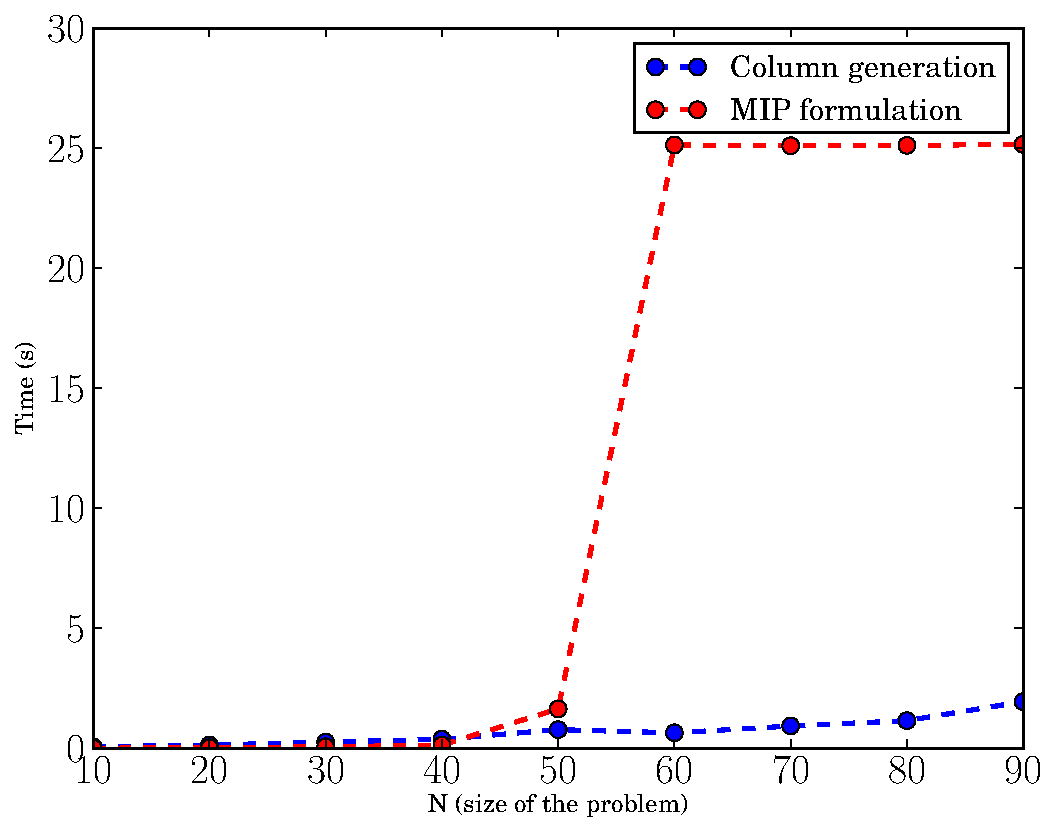
\includegraphics[width=0.8 \columnwidth]{colgen_results}
\caption{Comparison of runtimes for IP formulation and column generation for cutting stock problem. Note that the cost of the solution, i.e., the number of
rolls obtained by both the formulations was almost always the same. $N$ here is the total number of demands (generated randomly).}
\label{fig:csp_average_runtime}
\end{figure}

Let us show an example solution, for the problem setup in ~\eqref{eqn:eg_csp_small}, we get a solution which uses 13 rolls as
$$
[2,2,5],\ 2\times [2,7],\ 2 \times [3,6],\ [4,4],\ 5 \times [4,5],\ 2\times [8].
$$
This is indeed the optimal solution given by the IP formulation. The example in \eqref{eqn:eg_csp_big} has an optimal solution with 47 rolls. The code for
this problem can be seen at \href{https://github.com/pratikac/16.763/blob/master/extensions/column_generation/cutstock.py}{cutstock.py}
along with a generic branch and bound solver at
\href{https://github.com/pratikac/16.763/blob/master/extensions/column_generation/branch\_and\_bound.py}{branch\_and\_bound.py}.

\subsection{Resource-constrained shortest path (RCSP)}
\label{ssec:eg_shortest_path}

The RCSP problem is more interesting. An instance of a hand-drawn network is shown in Fig.~\ref{fig:rcsp}. For randomized tests, I generated a random road network as an Erdos-Renyi graph with probability of connection more than $0.5$ (this gives a connected graph almost surely). I picked an exponential random variable with mean $20$ as cost of each edge, while the time duration was sampled uniformly between $[10,20]$. An implementation of this problem is available at \href{https://github.com/pratikac/16.763/blob/master/extensions/column_generation/capacity.py}{capacity.py}, while the branch and price code is posted at \href{https://github.com/pratikac/16.763/blob/master/extensions/column_generation/capacity_bnb.py}{capacity\_bnb.py}.

The IP formulation is the same as shown in Prob.~\eqref{eqn:rcsp}. The details of column generation (cf. Prob.~\ref{eqn:rcsp_rlpm} for this problem are as follows --
\ilist{
    \item Generate the initial set of paths between the source and target node. I generated the set of all paths between these nodes, picked 4 paths randomly from among the ones which satisfy the constraints in \eqref{eqn:rcsp_resource} as the initial set of columns. Note that doing this in a large network is prohibitive, there are $\bigo(n!)$ paths in a network; one can use various depth-search heuristics to do this.
    \item The master problem is constructed using this set of columns while the sub-problem is a shortest path problem (with modified costs as shown in Eqn.~\eqref{eqn:rcsp_sub_problem}) and is solved using Dijkstra's algorithm. The solution of the sub-problem creates a new path that is added as a column in the master.
    \item I constructed an integral solution by adding the constraints from \eqref{eqn:rcsp_rlpm_flow} for binary $x_{ij}s$ into the relaxed master problem. This approach thus uses the columns obtained from column generation, but still solves the IP in Prob.~\ref{eqn:rcsp_rlpm}.
}

\textbf{\emph{Branch and price}:} Implementing branch and bound techniques for column generation is difficult, because often, one has to explicitly devise a good branching strategy. I implemented branch and price, i.e., branch and bound where each node is solved using column generation for RCSP using Alg.~\ref{alg:bnb} as follows.
\enum{
    \item We branch off on variables $x_{ij}$s in the IP formulation of the relaxed master. The crucial thing to note is that, since we fix particular values of $x_{ij}$, some paths in the set $P$ in Prob.~\ref{eqn:rcsp_rlpm} might become infeasible, in other words, there might be no way to satisfy constraint \eqref{eqn:rcsp_rlpm_flow} using the paths in $P$.
    \item One thus has to prune $P$ after branching, i.e., we maintain the set of variables $x_{ij}$s that are fixed (at that node in the branch and bound true), call this set $X_{bnb}$. We modify the set $P$ to be
    $$
    P' = \cbrac{p \in P: \forall (i,j) \in p, \not \exists\ x_{ij} = 0, x_{ij} \in X_{bnb}}
    $$
    and similarly for the edges that are set to 1,
    $$
    P^{''} = \cbrac{p \in P': \exists\ (i,j) \in p, x_{ij} = 1, x_{ij} \in X_{bnb}}.
    $$
    The modified set $P^{''}$ is used for column generation. It has a path $p$ if some $x_{ij} \in X_{bnb}$ on that path is fixed to 1 and removes all paths who have at least one $x_{ij} = 0$ on them.
}

\textbf{\emph{Results}:} Consider the network shown in Fig.~\ref{fig:rcsp}. By inspection, the optimal solution to Prob.~\eqref{eqn:rcsp} is the path $0-2-1-3-5$ to go from node $0$ to node $5$, and indeed the IP formulation gives this answer. The set $P$ considered by column generation with branch and price starts evolves as follows:
\aeqs{
    P_{init} = [0-2-1&-3-4-5],\ [0-2-1-3-5] \\
    P_1 &= P_{init} \cup [0-1-3-5]\\
    P_2 &= P_1 \cup [0-1-3-5]\\
    P_3 &= P_3 \cup [0-1-4-5]\\
    P_4 &= P_4 \cup [0-2-1-4-5].
}
Finally, we reach the optimal solution after 4 iterations and the cost is time duration is 13 for the path $0-2-1-3-5$.

We can also perform experiments on random networks. We first however need to pick a good value of the time constraint we shall use in \eqref{eqn:rcsp_resource}. I did this by computing all the paths in the network and using the median of time duration, i.e., about half of the $\bigo(n!)$ paths are candidate solutions for Prob.~\ref{eqn:rcsp_rlpm}.

\emph{Randomized instances} Using about 40 nodes in an Erdos-Renyi random graph with connectivity probability of 0.4 results in on an average (5 instances) 100,000 candidate paths. Column generation approach took 6 secs to execute on average. On the other hand, for this problem, the IP formulation running in parallel on 4 threads takes 10.6 secs per example.


\section{Summary}
\label{sec:summary}


{
\footnotesize
\bibliography{../writeup}
\bibliographystyle{alpha}
}
\end{document}
